\documentclass{article}
\usepackage[T2A]{fontenc} 
\usepackage[utf8]{inputenc} 
\usepackage[english,russian]{babel}
\usepackage{graphicx} 
\usepackage{amsmath}
\usepackage{amsfonts} 
\usepackage{titlesec}
\usepackage{listings}
\usepackage{float}
\usepackage{longtable}
\usepackage{titling} 
\usepackage{geometry} 
\usepackage{pgfplots}
\pgfplotsset{compat=1.9}
\usepackage{xcolor}
\definecolor{darkgreen}{RGB}{0,100,0}

\lstset{
  language=Python,
  basicstyle=\ttfamily,
  keywordstyle=\color{darkgreen},
  stringstyle=\color{purple},
  commentstyle=\color{green},
  morecomment=[l][\color{magenta}]{\#},
  frame=single, 
  showspaces=false, 
  showstringspaces=false, 
  numbers=left, 
  numberstyle=\tiny,
}

\titleformat{\section}
  {\normalfont\Large\bfseries}{\thesection}{1em}{}
\titleformat{\subsection}
  {\normalfont\large\bfseries}{\thesubsection}{1em}{}

\setlength{\droptitle}{-6em} 
\title{Отчет по лабораторной работе № 2 \\ Вариант № 3}
\author{Винницкая Дина Сергеевна}
\date{Группа: Б9122-02-03-01сцт}

\geometry{a4paper, margin=2cm}

\begin{document}

\maketitle
\section*{Цель работы}
\begin{enumerate}
    \item Построить таблицу конечных разностей по значениям
табличной функции.
    \item По соответствующим интерполяционным формулам вычислить значения
функции в заданных узлах
    \item Оценить минимум и макисмум для $f^{n + 1}(x)$
    \item Проверить на выполнение равенство $ \min{R_n} < R_n(z) < \max{R_n}$, где z - заданный угол, а $R_n(z) = L_n(z) - f(z)$
    \item Сделать вывод по проделанной работе.
\end{enumerate}

\section*{Входные данные:}
\begin{enumerate}

    \item \textbf{Функция:} $y=x^2 + \ln(x) - 4$
    \item \textbf{Отрезок} $[1.5,2.0]$
    \item $x^{*} = 1,52, \quad x^{**} = 1.52, \quad x^{***} = 1,97$
    
\end{enumerate}

\section*{Ход работы:}

\section{Используемые библиотеки}
Для реализации необходимой программы используются следующие библиотеки языка Python:

\begin{itemize}
    \item \textbf{PrettyTable} - библиотека $\textbf{Python}$PrettyTable предоставляет инструменты для создания красиво оформленных таблиц в $\textbf{Python}$. Она позволяет отображать данные в удобочитаемом виде, что упрощает их анализ и визуализацию.
    \begin{itemize}
        \item \textbf{Функциональность:} библиотека $\textbf{PrettyTable}$ обеспечивает возможность создания таблиц с различными стилями форматирования, включая плоские колонки, как в  $\textbf{PLAIN \_COLUMNS}$, что обеспечивает гибкость в представлении данных.
    \end{itemize}
\end{itemize}

\begin{itemize}
    \item \textbf{sympy} - библиотека $\textbf{sympy}$ представляет собой мощный символьный математический пакет для $\textbf{Python}$. Она способна обрабатывать символьные выражения, уравнения, и действия, что делает ее полезным инструментом в области научных вычислений, анализа данных и математического моделирования.
    \begin{itemize}
        \item \textbf{Функциональность:} библиотека $\textbf{sympy}$ позволяет выполнять различные операции с символами, такие как дифференцирование, интегрирование, решение уравнений и многое другое, что делает ее важным ресурсом для работы с математическими вычислениями в $\textbf{Python}$.
    \end{itemize}
\end{itemize}

\begin{lstlisting}
from prettytable import PrettyTable, PLAIN_COLUMNS
from sympy import *
\end{lstlisting}

\section{Инициализация входных данных}
Начиная реализацию алгоритма известна непосредственная функция$y=x^2 + \ln(x) - 4$ и отрезок $[1.5,2.0]$ \

\begin{lstlisting}
x = Symbol('x', real=True)
y = x**2 - log(x) - 4
a = 1.5
b = 2.0
h = (b - a) / 10
n = 11
x_star2 = 1.52
x_star3 = 1.52
x_star4 = 1.97
\end{lstlisting}

\begin{itemize}
\item В приведенном ниже коде определяется сама функция, границы отрезка, количество узлов для разбиения, $x^{*}, x^{**}, x^{***}$.
\end{itemize}

\section{Реализация непосредтвенного алгоритма}
Для реализации алгоритма были написаны следующие функции, позволяющие выполнить необходимый пласт работь, удовлетворить условию лабораторной работы и найти искомые значения. \\


\textbf{\large{Функция newton\_parameter\_minus}}

\begin{lstlisting}
def newton_parameter_minus(t: float, n: int):
    a = 1
    for i in range(n):
        a = a * (t - i)
    a = a / factorial(n)
    return a

\end{lstlisting}

\begin{itemize}
\item Функция \textbf{newton\_parameter\_minus(t: float, n: int)} 
Эта функция вычисляет параметр для метода Ньютона, используя отрицательные значения параметров.\\
\textbf{Алгоритм}
\begin{itemize}
    \item Инициализируется переменная \textbf{a} равная 1.
    \item Далее циклически умножается значение a на \textbf{(t - i)} для каждого значения \textbf{i} от 0 до n.
    \item Затем значение \textbf{a} делится на факториал \textbf{n}.
    \item Возвращается вычисленное значение параметра \textbf{a}

\end{itemize}
\end{itemize}


\textbf{\large{Функция newton\_parameter\_plus}}
\begin{lstlisting}
def newton_parameter_plus(t: float, n: int):
    a = 1
    for i in range(n):
        a = a * (t + i)
    a = a / factorial(n)
    return a

\end{lstlisting}

\begin{itemize}
\item Функция \textbf{newton\_parameter\_plus(t: float, n: int)} 
Данная функция вычисляет параметр для метода Ньютона с использованием положительных параметров. \\
\textbf{Алгоритм}
\begin{itemize}
    \item Инициализируется переменная \textbf{a} равная 1.
    \item Далее циклически умножается значение a на \textbf{(t + i)} для каждого значения \textbf{i} от 0 до n.
    \item Затем значение \textbf{a} делится на факториал \textbf{n}.
    \item Функция возвращает вычисленное значение параметра \textbf{a}

\end{itemize}
\end{itemize}

\vspace{5\baselineskip}


\textbf{\large{Функция gauss1\_minus}}
\begin{lstlisting}
def gauss1_minus(t: float, n: int):
    a = 1
    for i in range(n):
        if i % 2 == 1 or i == 0:
            a = a * (t - i)
        else:
            a = a * (t + i - 1)
    a = a / factorial(n)
    return a

\end{lstlisting}
\begin{itemize}
\item Функция \textbf{gauss1\_minus(t: float, n: int)} 
Эта функция рассчитывает параметр для метода Гаусса с отрицательными параметрами.\\
\textbf{Алгоритм}
\begin{itemize}
    \item Инициализируется переменная \textbf{a} равная 1.
    \item В цикле вычисляется значение параметра \textbf{a}, учитывая условия для умножения на \textbf{(t - i) и (t + i - 1)} в зависимости от значения \textbf{i}.
    \item Функция возвращает вычисленное значение параметра \textbf{a}

\end{itemize}
\end{itemize}

\textbf{\large{Функция gauss2\_plus}}
\begin{lstlisting}
def gauss2_plus(t: float, n: int):
    a = 1
    for i in range(n):
        if i % 2 == 1 or i == 0:
            a = a * (t + i)
        else:
            a = a * (t - i + 1)
    a = a / factorial(n)
    return a
\end{lstlisting}

\begin{itemize}
\item Функция \textbf{gauss2\_plus(t: float, n: int)} 
Эта функция вычисляет параметр для метода Гаусса с положительными параметрами.\\
\textbf{Алгоритм}
\begin{itemize}
    \item Инициализируется переменная \textbf{a} равная 1.
    \item В цикле вычисляется значение параметра \textbf{a}, учитывая условия для умножения на \textbf{(t + i) и (t - i + 1)} в зависимости от значения \textbf{i}.
    \item Функция возвращает вычисленное значение параметра \textbf{a}

\end{itemize}
\end{itemize}


\textbf{\large{Функция insert\_gauss1}}
\begin{lstlisting}
def insert_gauss1(t: float, n: int, mass: list):
    Px = 0
    j = 5
    for i in range(n):
        Px += mass[i][j] * gauss1_minus(t, i)
        if i % 2 != 0:
            j -= 1
    return Px
\end{lstlisting}

\begin{itemize}
\item Функция \textbf{insert\_gauss1(t: float, n: int, mass: list)} 
Данная функция вставляет метод Гаусса с отрицательными параметрами.\\
\textbf{Алгоритм}
\begin{itemize}
    \item Переменная \textbf{Px} инициализируется как 0.
    \item Производятся вычисления с использованием метода \textbf{gauss1Minus} для вычисления значения \textbf{Px}.
    \item Возвращается результат вычисления \textbf{Px}.

\end{itemize}
\end{itemize}


\textbf{\large{Функция insert\_gauss2}}
\begin{lstlisting}
def insert_gauss2(t: float, n: int, mass: list):
    Px2 = 0
    j = 5
    for i in range(n):
        Px2 += mass[i][j] * gauss2_plus(t, i)
        if i % 2 == 0:
            j -= 1
    return Px2
\end{lstlisting}

\begin{itemize}
\item Функция \textbf{insert\_gauss2(t: float, n: int, mass: list)} 
Эта функция вставляет метод Гаусса с положительными параметрами.\\
\textbf{Алгоритм}
\begin{itemize}
    \item Переменная \textbf{Px2} инициализируется как 0.
    \item Производятся вычисления с использованием метода \textbf{gauss2Plus} для вычисления значения \textbf{Px2}.
    \item Возвращается результат вычисления \textbf{Px2}.

\end{itemize}
\end{itemize}

\textbf{\large{Функция insert\_newton1}}
\begin{lstlisting}
def insert_newton1(t: float, n: int, mass: list):
    Px = 0
    j = 0
    for i in range(n):
        Px += mass[i][j] * newton_parameter_minus(t, i)
    return Px
\end{lstlisting}

\begin{itemize}
\item Функция \textbf{insert\_newton1(t: float, n: int, mass: list)} 
Данная функция вставляет метод Ньютона с отрицательными параметрами.\\
\textbf{Алгоритм}
\begin{itemize}
    \item Переменная \textbf{Px} инициализируется как 0.
    \item Производятся операции с использованием метода \textbf{newton\_parameterMinus} для вычисления \textbf{Px}.
    \item Возвращается результат вычисления \textbf{Px}.

\end{itemize}
\end{itemize}

\textbf{\large{Функция insert\_newton2}}
\begin{lstlisting}
def insert_newton2(t: float, n: int, mass: list):
    Px2 = 0
    for i in range(0, n):
        j = n - i - 1
        Px2 += mass[i][j] * newton_parameter_plus(t, i)
    return Px2
\end{lstlisting}

\begin{itemize}
\item Функция \textbf{insert\_newton2(t: float, n: int, mass: list)} 
Эта функция вставляет метод Ньютона с положительными параметрами.\\
\textbf{Алгоритм}
\begin{itemize}
    \item Переменная \textbf{Px2} инициализируется как 0.
    \item Производятся операции с использованием метода \textbf{newton\_parameterPlus} для вычисления \textbf{Px2}.
    \item Возвращается результат вычисления \textbf{Px2}.

\end{itemize}
\end{itemize}

\section{Нахождение значений}
\textbf{\large{Таблица значений функции y(x)}}

\begin{lstlisting}
x_list = []
y_list = []
for i in range(0, 11):
    xi = a + i * h
    x_list.append(xi)
    yi = y.subs(x, xi).evalf()
    y_list.append(yi)
table.add_column("№", [i for i in range(0, 11)])
table.add_column("x", x_list)
table.add_column("y(x)", y_list)
print(table)
\end{lstlisting}

\begin{itemize}
    \item Цикл for проходит по значениям от 0 до 10.
    \item Для каждого значения i вычисляется xi как сумма a и произведение i на h.
    \item Значение \textbf{xi} добавляется в список \textbf{x\_list}.
    \item Значение \textbf{yi} вычисляется с использованием функции \textbf{subs} для подстановки  \textbf{xi} вместо переменной \textbf{x} в функцию \textbf{y}, а затем вычисляется численное значение с помощью  \textbf{$evalf()$}.
    \item Значение \textbf{yi} добавляется в список \textbf{y\_list}.

\end{itemize}

Создание таблицы, которая способна наглядно показать визуально оценить изменение функции для различных значений \textbf{x}. Это обеспечивает наглядное представление данных и упрощает анализ поведения функции на определенном диапазоне. 

\begin{figure}[h]
    \centering
    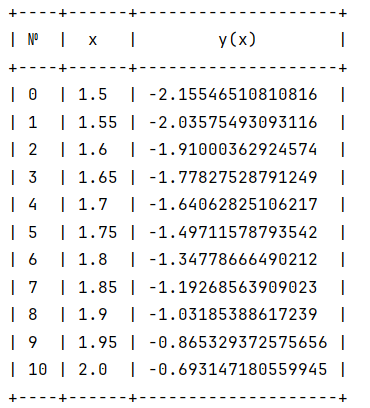
\includegraphics[width=0.5\textwidth]{t_lab_2_1.png}
    \caption{Таблица значений функции y(x)}
    \label{fig:my_label}
\end{figure}


\vspace{18\baselineskip}

\textbf{\large{Расчет разностей и формирование новой таблицы}}

\begin{lstlisting}
list_diffs = [y_list.copy()]

while len(list_diffs[-1]) != 1:
   lis = []
   for i in range(0, len(list_diffs[-1]) - 1):
       lis.append(list_diffs[-1][i + 1] - list_diffs[-1][i])
   list_diffs.append(lis)

list_to_table = list_diffs.copy()
max_length = len(max(list_to_table, key=len))

for lst in list_to_table:
   while len(lst) < max_length:
       lst.append("")

table.field_names = ["№", "Value 1", "Value 2", "Value 3", "Value 4",
"Value 5", "Value 6", "Value 7", "Value 8",
                        "Value 9", "Value 10", "Value 11"]
for i in range(0, len(list_to_table)):
   table.add_row([f"{i}"] + list_to_table[i])

table.set_style(PLAIN_COLUMNS)
print(table)

\end{lstlisting}

Эта таблица представляет собой таблицу разностей, которая является инструментом для вычисления и визуализации разностей между последовательными значениями в исходном наборе данных. 

\begin{table}[H]
\centering
\begin{tabular}{|c|c|c|c|c|}
\hline
№ & Value 1 & Value 2 & Value 3 & Value 4 \\ \hline
0 & -2.15546510810816 & -2.03575493093116 & -1.91000362924574 - 1.77827528791249 & -1.64062825106217 \\ \hline
1 & 0.119710177177009 & 0.125751301685420 & 0.131728341333246 & 0.137647036850319 \\ \hline
2 & 0.00604112450841043 & 0.00597703964782581 & 0.00591869551707314 & 0.00586542627642905 \\ \hline
3 & -6.40848605846234e-5 & -5.83441307526744e-5 & -5.32692406440827e-5 & -4.87663631655e-5 \\ \hline
4 & 5.74072983194895e-6 & 5.07489010859175e-6 & 4.50287077091716e-6 & 4.00924189913887e-6 \\ \hline
\end{tabular}
\\[10pt]
\begin{tabular}{|c|c|c|c|c|}
\hline
№ & Value 5 & Value 6 & Value 7 & Value 8 \\ \hline
0 & -1.49711578793542 & -1.34778666490212 & -1.19268563909023 & -1.03185388617239 \\ \hline
1 & 0.143512463126748 & 0.149329123033304 & 0.155101025811886 & 0.160831752917838 \\ \hline
2 & 0.00581665990655589 & 0.00577190277858186 & 0.00573072710595257 & 0.00569276067890101 \\ \hline
3 & -4.47571279740266e-5 & -4.11756726292900e-5 & -3.79664270515612e-5 & -3.50822599298750e-5 \\ \hline
4 & 3.58145534473664e-6 & 3.20924557772884e-6 & 2.88416712168615e-6 &  \\ \hline
\end{tabular}
\\[10pt]
\begin{tabular}{|c|c|c|c|c|}
\hline
№ & Value 9 & Value 10 & Value 11 \\ \hline
0 & -0.865329372575656 &  &  \\ \hline
1 & 0.166524513596739 & 0.172182192015710 &  \\ \hline
2 & 0.00565767841897113 &  &  \\ \hline
3 &  &  &  \\ \hline
4 &  &  &  \\ \hline
\end{tabular}
\end{table}



\textbf{\large{Вычисление параметров методов и их погрешностей}} \\ 
На этапе вычисления параметров методов и оценки их погрешностей происходит ключевой анализ результатов и определение точности методов Ньютона и Гаусса. Происходит расчет параметров, необходимых для осуществления методов численного анализа, а также оценка погрешностей этих методов. \\
В процессе вычисления параметров методов Ньютона и Гаусса рассчитываются значения параметров \textbf{t} и \textbf{t1}, \textbf{t2}, которые используются для правильного применения соответствующих методов численного дифференцирования. Далее происходит вызов функций для данных методов, а также вычисление и анализ погрешностей этих методов \\ \\ \\ \\ \\ \\ \\ \\ 

\begin{lstlisting}
t = min(abs(x_list[0] - x_star2), abs(x_list[1] - x_star2)) / h

print('N 1:', insert_newton1(t, 11, list_diffs))
print("R_N1: ", insert_newton1(t, 11, list_diffs) - 
y.subs(x, x_star2).evalf())

t = -1 * (x_list[-1] - x_star3) / h

print('N 2:', insert_newton2(t, 11, list_diffs))
print("R_N2: ", insert_newton2(t, 11, list_diffs) -
y.subs(x, x_star3).evalf())

i = 0
for i in range(n - 1):
    if (x_list[i] < x_star4) and (x_list[i + 1] > x_star4):
        break

t1 = abs(x_list[i] - x_star4) / h
t2 = abs(x_list[i + 1] - x_star4) / h

if t1 < t2:
    print('G 1:', insert_gauss1(t1, 11, list_diffs))
    print("R_G1: ", insert_gauss1(t1, 11, list_diffs) -
    y.subs(x, x_star4).evalf())
else:
    t2 = -1 * t2
    print('G 2:', insert_gauss2(t2, 11, list_diffs))
    print("R_G2: ", insert_gauss2(t2, 11, list_diffs) - 
    y.subs(x, x_star4).evalf())

w = 1
for i in range(11):
    w = w * (x - x_list[i])

y_der = diff(y, x, n + 1)
R_n = y_der * w / factorial(n + 1)

crit_points = solve(y_der, x)
crit_points = [point for point in crit_points if a <= float(point) <= b]
endpoints = [a, b]
values_at_endpoints = {endpoint: y_der.subs(x, endpoint).evalf() 
for endpoint in endpoints}
values_at_critical_points = {cp: y_der.subs(x, cp).evalf() 
for cp in crit_points}
extremum_values = list(values_at_endpoints.values()) +
list(values_at_critical_points.values())
\end{lstlisting} 
\textbf{Реализация} \\
\textbf{1. Вычисление параметров для метода Ньютона:}
\begin{itemize}
    \item Вычисляется значение $ \mathbf{t} $ для метода Ньютона 1, которое представляет собой минимальное из двух значений: разницы между нулевым элементом списка $ \mathbf{x\_list} $ и $ \mathbf{x\_star2} $, и разницы между первым элементом списка $ \mathbf{x\_list} $ и $ \mathbf{x\_star2} $, деленное на $ \mathbf{h} $.
    \item Далее при помощи функций \texttt{insert\_newton1} и \texttt{insert\_newton2} происходит вычисление метода и его оценка.
\end{itemize}

\textbf{2. Вычисление параметров для метода Гаусса:}
\begin{itemize}
    \item Вычисляются значения $ \mathbf{t1} $ и $ \mathbf{t2} $ для метода Гаусса, представляющие собой отношение модуля разности между определенными значениями из $ \mathbf{x\_list} $ и $ \mathbf{x\_star4} $ к $ \mathbf{h} $.
    \item В зависимости от соотношения $ \mathbf{t1} $ и $ \mathbf{t2} $, вызываются функции \texttt{insert\_gauss1} или \texttt{insert\_gauss2} для расчета метода Гаусса и оценки его погрешности.
\end{itemize}

\textbf{3. Подготовка данных для дальнейшего анализа:}
\begin{itemize}
    \item Выполняется вычисление произведения $ (x - \mathbf{x\_list[i]}) $ для всех элементов $ \mathbf{x\_list} $.
\end{itemize}

\textbf{4. Расчет критических точек и их значений:}
\begin{itemize}
    \item Производная $ \mathbf{y\_der} $ функции $ \mathbf{y} $ вычисляется по $ \mathbf{x} $ до $ (n + 1) $ порядка.
    \item Проводится поиск критических точек на отрезке между $ \mathbf{a} $ и $ \mathbf{b} $.
    \item Значения производной на конечных точках и на критических точках вычисляются и сохраняются в соответствующих словарях.
\end{itemize}
\textbf{Вывод}

\begin{figure}[h]
    \centering
    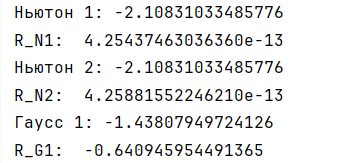
\includegraphics[width=0.5\textwidth]{lab_2_2.png}
    \caption{Значение точек экстремума}
    \label{fig:my_label}
\end{figure}

\begin{itemize}
\item Исходя из полученных данных, можно сделать следующие выводы: 
\begin{itemize}
    \item Значения и оценки для обоих вариантов метода Ньютона близки друг к другу, что говорит о сходимости метода.
    \item Значение Гаусса и его оценка также близки, что указывает на надежность результатов метода.
    \item Основываясь на полученных данных, можно заключить, что и метод Ньютона, и метод Гаусса дали близкие значения и оценки, что свидетельствует о их эффективности и точности.

\end{itemize}

\section*{Поиск значений и оценка точек экстремума}

Этапы поиска значений точек экстремума является важным этапом в анализе функций и моделей.

\textbf{1. Производные функции:}
\begin{itemize}
    \item Для поиска точек экстремума сначала вычисляются производные функций. Это может быть первая производная для определения точек экстремума первого порядка или высшие производные для точек экстремума более высокого порядка.
\end{itemize}

\textbf{2. Решение уравнений:}
\begin{itemize}
    \item Затем производные приравниваются к нулю, чтобы найти критические точки, где производная равна нулю. Решение уравнения производной равной нулю позволяет найти потенциальные точки экстремума.
\end{itemize}

\textbf{3. Определение интервала:}
\begin{itemize}
    \item После нахождения критических точек необходимо оценить интервал, в котором следует искать точки экстремума, обычно между двумя критическими точками или в пределах определенного диапазона.
\end{itemize}

\textbf{4. Вычисление значений:}
\begin{itemize}
    \item Затем вычисляются значения функции в найденных критических точках, а также на конечных точках заданного интервала, что позволяет определить, являются ли найденные точки минимумами или максимумами.
\end{itemize}

\textbf{5. Оценка экстремума:}
\begin{itemize}
    \item Для оценки экстремума сравниваются значения функции в найденных точках, определяется минимальное и максимальное значение. Это позволяет определить, где находятся точки минимума и максимума на заданном интервале.
\end{itemize}


\begin{lstlisting}
w = 1
for i in range(11):
    w = w * (x - x_list[i])

y_der = diff(y, x, n + 1)
R_n = y_der * w / factorial(n + 1)

crit_points = solve(y_der, x)
crit_points = [point for point in crit_points if a <= float(point) <= b]

values_at_endpoints = {endpoint: y_der.subs(x, endpoint).evalf()
for endpoint in endpoints}
values_at_critical_points = {cp: y_der.subs(x, cp).evalf()
for cp in crit_points}

extremum_values = list(values_at_endpoints.values()) + 
list(values_at_critical_points.values())

minimum = min(extremum_values)
maximum = max(extremum_values)
print('Min f(12)(E):', minimum)
print('Max f(12)(E):', maximum)

crit_points = solve(R_n, x)
crit_points = [point for point in crit_points if a <= float(point) <= b]

values_at_endpoints = {endpoint: R_n.subs(x, endpoint).evalf()
for endpoint in endpoints}

values_at_critical_points = {cp: R_n.subs(x, cp).evalf()
for cp in crit_points}

extremum_values = list(values_at_endpoints.values()) +
list(values_at_critical_points.values())

minimum = min(extremum_values)
maximum = max(extremum_values)
print('Min Rn:', minimum)
print('Max Rn:', maximum)
\end{lstlisting}

\begin{figure}[h]
    \centering
    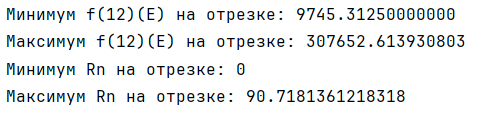
\includegraphics[width=0.5\textwidth]{lab_2_3.png}
    \label{fig:my_label}
\end{figure}

Исходя из полученных данных, можно сделать следующие выводы относительно поведения функции:

1. \textbf{Поведение функции f(12)(E)}: \\
   - Минимум функции f(12)(E) на отрезке составляет 9745.31250000000, что указывает на точку, в которой функция достигает своего наименьшего значения на данном отрезке. \\
   - Максимум функции f(12)(E) на отрезке равен 307652.613930803, показывая точку экстремума, в которой функция достигает своего наивысшего значения на заданном отрезке. \\
   - Эти значения отражают изменения функции f(12)(E) в пределах заданного диапазона и могут быть важными при анализе ее поведения.

2. \textbf{Оценка Rn и поведение}: \\
   - Минимальное значение оценки Rn на отрезке равно 0, что может указывать на минимальное воздействие погрешностей на результаты функции на данном отрезке. \\
   - Максимальное значение оценки Rn на отрезке составляет 90.7181361218318, что отражает максимальное воздействие погрешностей на результаты функции в заданном диапазоне. \\


\section*{Проверка равенства}
\begin{figure}[h]
    \centering
    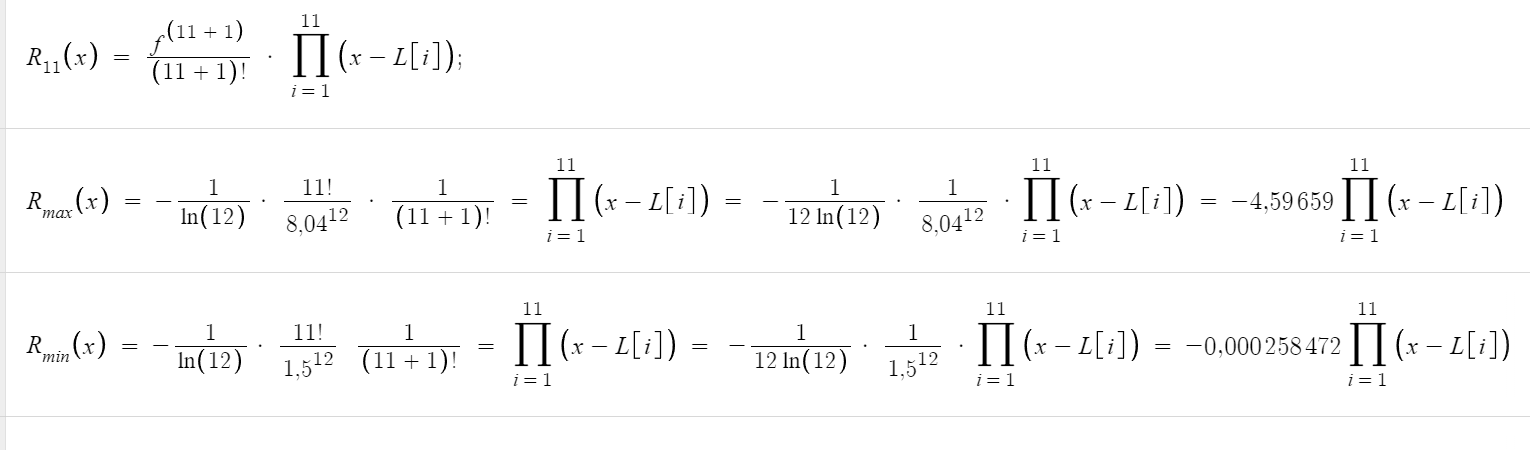
\includegraphics[width=0.7\textwidth]{lab_2_4.png}
    \label{fig:my_label}
\end{figure}
Максимальное значение $R_n$ равно -4.59659, а минимальное значение $R_n$ равно -0.000258472. Исходя из этого, можно сделать вывод, что неравенство $\min{R_n} < R_n(z) < \max{R_n}$ выполняется для всех значений $R_n(z)$ в интервале от минимального до максимального значения.

Это означает, что условие $\min{R_n} < R_n(z) < \max{R_n}$ соблюдается для всех $R_n(z)$ и подтверждает то, что значения $R_n(z)$ находятся в соответствующем интервале между минимальным и максимальным значениями $R_n$.
\section*{Вывод}

В ходе выполнения лабораторной работы были реализованы различные численные методы (методы Ньютона и методы Гаусса) для аппроксимации функции.

\begin{enumerate}
    \item \textbf{Входные данные:}
    \begin{itemize}
        \item функция $y = x^2 - \log(x) - 4$.
        \item Отрезок [$a = 1.5$, $b = 2.0$] и шаг разбиения ($h = \frac{b - a}{10}$).
    \end{itemize}

    \item \textbf{Применение методов аппроксимации:}
    \begin{itemize}
        \item Методами Ньютона и Гаусса были найдены коэффициенты аппроксимирующих многочленов.
        \item Были примены методы для вычисления значений аппроксимирующих многочленов в заданных точках.
    \end{itemize}

    \item \textbf{Анали результатов:}
    \begin{itemize}
        \item Были найдены минимальное и максимальное значение $R_{n}$ на заданном интервале.
        \item Произведено сравнение результатов и проверка неравенства $\min{R_n} < R_n(z) < \max{R_n}$.
    \end{itemize}
\end{enumerate}

\textbf{\large{}} \\ 

\thispagestyle{empty} 
\newpage
\mbox{}
\thispagestyle{empty} 
\newpage
 
\end{document}
